
\chapter{Introduction into copulae}

\label{Chapter1}

\section{Motivation}

A copula is a bi- or multivariate distribution function, that allows to model dependency between variables with arbitrary marginal distributions. It has, therefore, become a handy tool in risk and portfolio analysis but also in geology and hydrology as the joint behavior of arbitrarily distributed variables can be modeled precisely. Apart from the empirical copula, all copulae are parameterized by either one, or two parameters that allows them to be fit to practically any desired dependence structure. The efficient estimation of a copula's parameter or the selection of a suitable copula itself is subject to current research. For this study I use a novel approach for selecting a copula given a set of data, using two computationally efficient moment-based estimators in combination with Akaike's Information Criterion, to achieve maximum-likelihood-like accuracy with only $1/16^{th}$ the computational effort.

The rest of this article is organized as follows. The first chapter gives an introduction into copulae itself, and how they are defined. Chapter two details the estimation methods used in this Monte-Carlo study while chapter three carries out the study and concludes.

\section{Copula existence and Sklar's theorem}

At the very heart of copula theory is the theorem of \citet{sklar1959} stating that any multivariate distribution can be decomposed into its univariate margins and a copula, which captures the dependence between variables. Therefore, let $\mathbf{X}=\left(X_1,\dots,X_d\right)^{\top}$ be a $d$-dimensional random vector with joint distribution $F$ and marginal distributions $F_{X_1},\dots, F_{X_d}$. Now, for every realization $\mathbf{x}=\left(x_1,\dots,x_d\right)^{\top} \in \left[-\infty,\infty\right]^{d}$,

\begin{equation}
	\label{sklar}
	\begin{split}
		F(\mathbf{x})&=C\left(F_{X_1}(x_1),\dots, F_{X_d}(x_d)\right)\\
		&= P(X_1 < x_1, \dots, X_d < x_d),
	\end{split}
\end{equation}
%
where the copula $C$ can be interpreted as a $d$-dimensional distribution function defined on the unit hypercube $C:[0,1]^{d} \rightarrow [0,1]$ with uniformly distributed marginals (see \citet{angus1994probability} for proof). If all $F_{\mathbf{X}}$ are continuous $C$ is unique.

The inverse theorem also holds: If $\mathbf{u} \equiv \left(u_1,\dots,u_d\right)^{\top} \in [0,1]^{d}$ and $u_i = F_{X_i}(x_i)$ for $i = 1, \dots , d$ the copula $C$ can be expressed as

\begin{equation}
	\label{copula_def}
	C\left(\mathbf{u}\right)=F\left(F_{X_1}^{-1}\left(u_{1}\right), \ldots, F_{X_d}^{-1}\left(u_{d}\right)\right), 
\end{equation}
%
with the corresponding multivariate distribution $F$, marginal distributions $F_{\mathbf{X}}$ and inverses $F^{-1}$, given their existence \citep{durante2013topological}. Furthermore, using the relationship between density functions and distribution functions and their partial derivatives, the multivariate joint density can be expressed as the product of the copula density and the marginal densities

\begin{equation}
	f\left(\mathbf{x}\right)=c\left(F_{X_1}\left(x_{1}\right), \ldots, F_{X_d}\left(x_{d}\right)\right) f_{X_1}\left(x_{1}\right) \ldots f_{X_d}\left(x_{d}\right),
\end{equation}
%
with the copula density $c$ being derived as $c=\frac{\partial C(\mathbf{u})}{\partial \mathbf{u}}$.

%-----------------------------------
%	SUBSECTION 1
%-----------------------------------
\section{Selected copulae and properties}

Since their discovery a variety of copula functions have been constructed for different purposes. There are only few Archimedean copulae defined for $d\geq 2$, therefore we will  stick to bivariate representations for this simulation. This is sufficient as there is a concept - the Pair-Copula-Construction (PCC) - that allows to model multivariate problems by splitting them into several tow-dimensional ones and solving them consecutively. 

There are two major classes of copulae distinguished by how they are generated:

%-----------------------------------
%	SUBSECTION 2
%-----------------------------------

\subsection{Elliptical copulae}

Following equation \ref{copula_def} a copula $C$ is elliptical if $F$ is elliptical, meaning its density can be represented by

\begin{equation}
	f(\mathbf{x}; \boldsymbol{\mu},\Sigma)=k_{d}|\Sigma|^{-\frac{1}{2}} g\left((\mathbf{x}-\boldsymbol{\mu})^{\top} \Sigma^{-1}(\mathbf{x}-\boldsymbol{\mu})\right),
\end{equation}
%
with some constant $k_{d} \in \mathbb{R}$ dependent on the dimension, a vector of means $\boldsymbol{\mu} \in \mathbb{R}^{d}$, a symmetric positive definite matrix $\Sigma \in \mathbb{R}^{d\times d}$ and some function $g: \mathbb{R}_{0}^{+} \rightarrow \mathbb{R}_{0}^{+}$ which is independent of the dimension $d$. One prominent example of a copula derived from elliptical distributions is the $d$-variate Gaussian copula, 

\begin{equation}
	C\left(\mathbf{u}; \Sigma\right)=\Phi_{\Sigma}^{d}\left(\Phi^{-1}\left(u_{1}\right), \dots \Phi^{-1}\left(u_{d}\right)\right),
\end{equation}
%
where $\Phi (\cdot)$ is the standard normal distribution function $N(0,1)$ and $\Phi_{\Sigma}^{d} (\cdot,\dots,\cdot)$ being the $d$-variate normal distribution function with zero means, unit variances and correlation matrix $\Sigma$.

The Gaussian copula had been widely used in finance to model the joint default risk of portfolios containing different asset classes. This, however, led to an underestimation of defaulting risks as the phenomenon of dependent extreme values, which is often observed in financial return data cannot be modeled using this copula (see \citet{salmon2012formula} for a popular science article about this misconception and its effects on the financial crisis of 2007).

Many recent paper (\citet{mashal2003dependence}, \citet{breymann2003dependence} or \citet{lucas2014conditional}) therefore use the $t$-copula which resembles the dependence structure implicit in a multivariate $t$-distribution as it is able to better capture extreme value dependence due to its heavy tails. The $d$-variate $t$-copula is defined as

\begin{equation}
	C(\mathbf{u}; R, \nu)=T_{R, \nu}\left(T_{\nu}^{-1}\left(u_{1}\right),\dots, T_{\nu}^{-1}\left(u_{d}\right)\right),
\end{equation}
%
where $T_{R, \nu}$ denotes the multivariate students $t$-distribution with density

\begin{equation}
	f(\mathbf{x})=\frac{\Gamma\left(\frac{\nu+d}{2}\right)}{\Gamma\left(\frac{\nu}{2}\right) (\pi \nu)^{\frac{d}{2}}}|R|^{-\frac{1}{2}}\left(1+\frac{(\mathbf{x}-\mu)^{\top} R^{-1}(\mathbf{x}-\mu)}{\nu}\right)^{\frac{-\nu+d}{2}},
\end{equation}
%
scale matrix $R \in \left[ -1,1\right]^{d\times d}$ and the degrees of freedom $\nu > 0$. $T_{\nu}^{-1}$ represents the quantile function of the univariate students $t$- distribution with the same $\nu > 0$ degrees of freedom (see \citet{demarta2005t} for a more detailed description). Figure \ref{dens-cont-normal-t} shows the two just presented copulae for some visual intuition.

\begin{figure}[!ht]
	\subfloat{%
		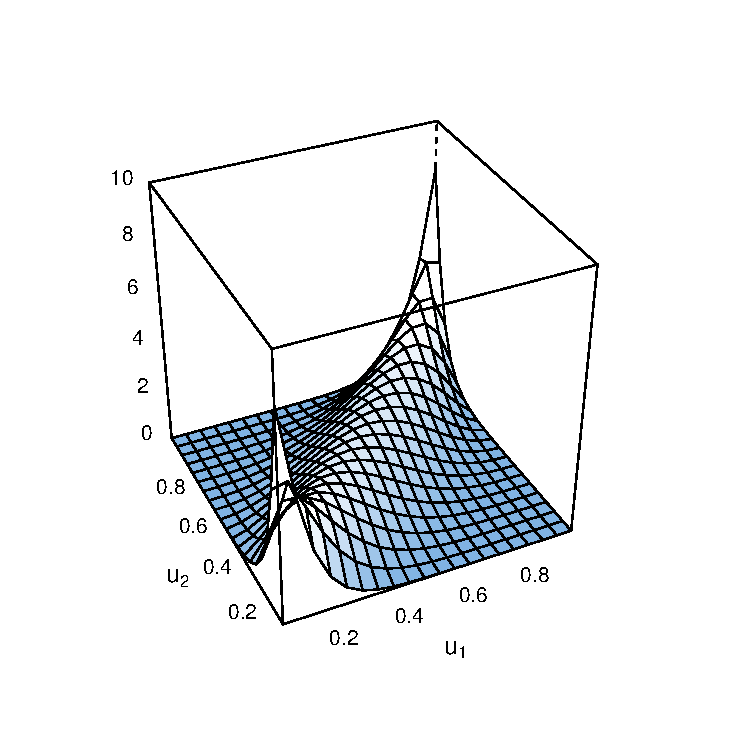
\includegraphics[trim= 1cm 1cm 2cm 1cm, clip=true, width = .5\textwidth]{Figures/Fig-1-1/gaussian-copula.pdf}
	}
	\hfill
	\subfloat{%
		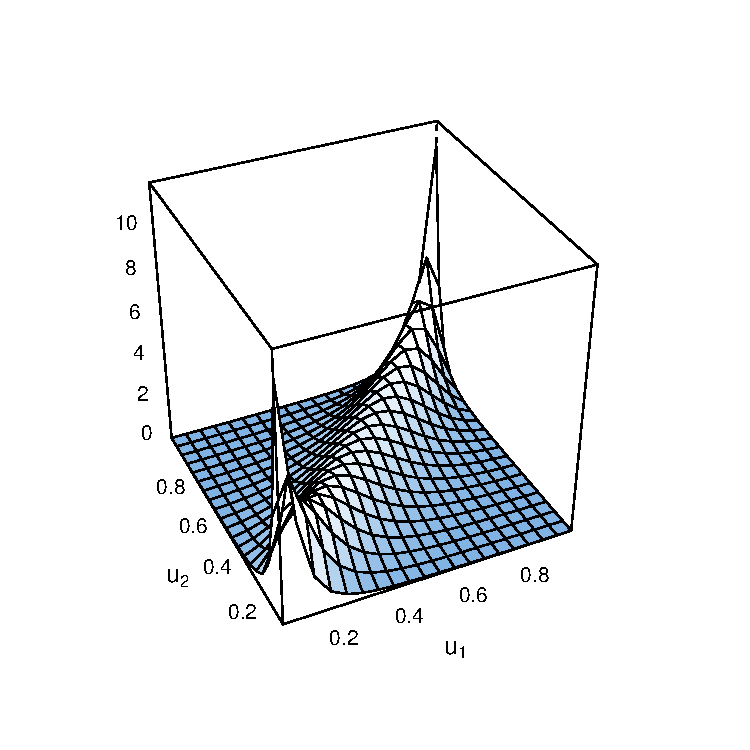
\includegraphics[trim= 1cm 1cm 2cm 1cm, clip=true, width = .5\textwidth]{Figures/Fig-1-1/t-copula.pdf}
	}
	\hfill
	\subfloat{%
		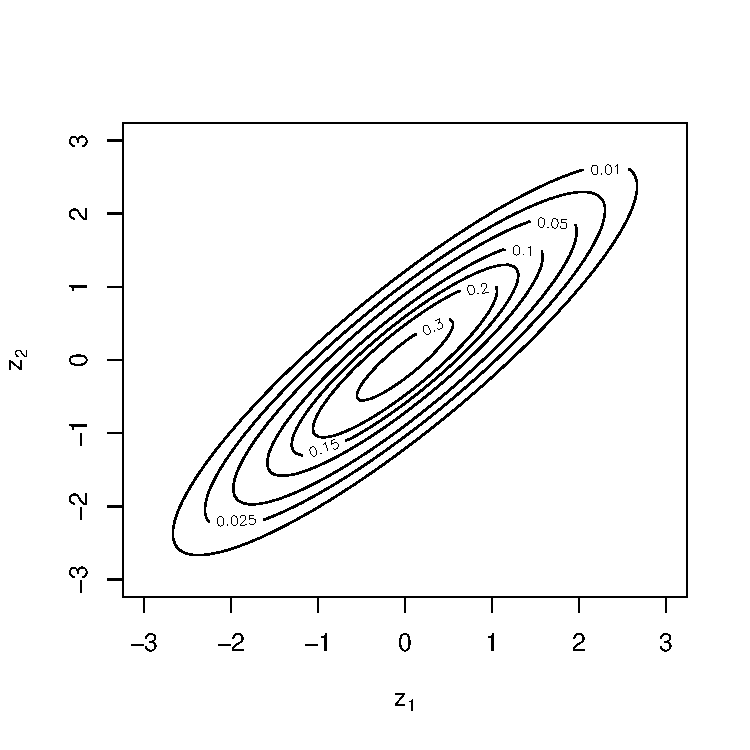
\includegraphics[trim= 0cm 0cm 0cm 2cm, clip=true, width = .5\textwidth]{Figures/Fig-1-1/gauss-contour.pdf}
	}
	\hfill
	\subfloat{%
		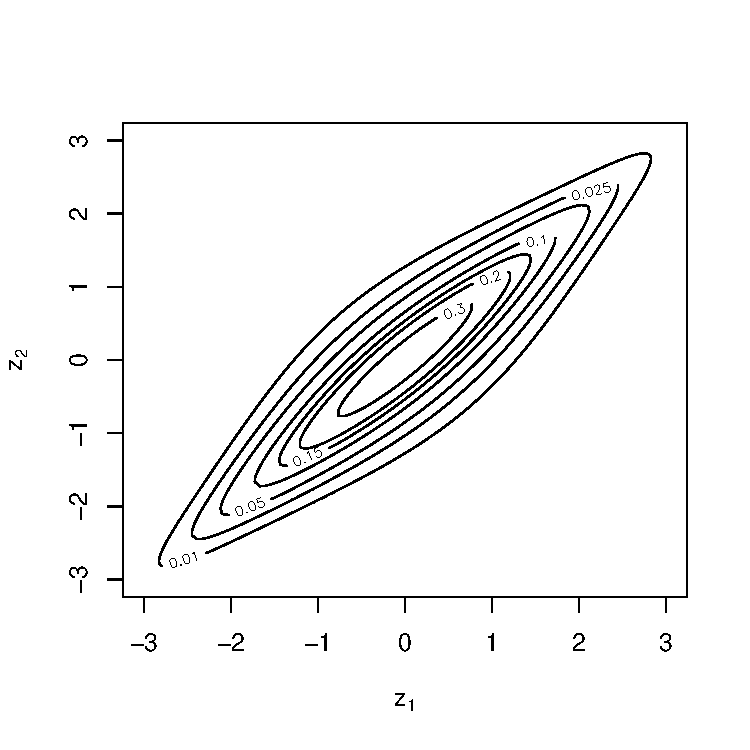
\includegraphics[trim= 0cm 0cm 0cm 2cm, clip=true, width = .5\textwidth]{Figures/Fig-1-1/t-contour.pdf}
	}
	\caption[\textsc{Bivariate elliptical copula densities:} A comparison between Gaussian and $t$-copulae]{\textsc{Bivariate elliptical copula densities:} Top: three-dimensional density plots of a theoretical Gaussian copula (left) and a $t$-copula with $\nu = 4$ degrees of freedom (right). The parameters have been chosen in such a way that Kendall's $\tau = 0.7$. Below are the respective contour plots belonging to the densities. The plots were generated using the BiCop function from the VineCopula package in R.}
	\label{dens-cont-normal-t}
\end{figure}

\subsection{Archimedean copulae}

Archimedean copulae and their detailed properties have already been discussed by for example \citet{nelsen2007introduction} or \citet{mcneil2009multivariate}. Therefore, we now derive just the fundamental building blocks for bivariate Archimedean copulae.

Following the work of \citet{genest1993statistical} a copula is called \textit{Archimedean} if it can be expressed as

\begin{equation}
	C_{\varphi}\left( \mathbf{u}\right) = \varphi ^{[-1]}\left( \varphi \left( u_1\right) +\dots +\varphi \left( u_d\right) \right),
\end{equation}
%
for some continuous, strictly monotone decreasing, and convex function $\varphi : \mathbf{I} \rightarrow \left[ 0,\infty \right] $, satisfying $\varphi \left( 1 \right)=0$ and $\mathbf{I}$ being the unit interval. This function is called the \textit{generator function} for the copula and is furthermore called \textit{strict} if $\varphi \left( 0 \right) = \infty$. $\varphi ^{[-1]}$ is the pseudo-inverse satisfying the following conditions

\begin{equation}
	\varphi^{[-1]}(t):=\left\{\begin{array}{ll}
		\varphi^{-1}(t)&, 0 \leq t \leq \varphi(0) \\
		0 & , \varphi(0) \leq t \leq \infty .
	\end{array}\right.
\end{equation}

We will now present the Archimedean copulae with its generators and properties that this simulation study will use. To date there has been defined a wide variety of Archimedean copulae with contrasting properties (see \citet{nelsen2007introduction} for a comprehensive list).

For $\varphi_\theta \left( u\right) = \left(- \log\left(u \right)\right)^{\theta} $ with $\theta \in \left[ 1,\infty\right) $ we attain the Gumbel copula. We include it in this simulation because it is representative for the subclass of asymmetric tail dependent copulae (upper tail dependence only) while the Gaussian and $t$-copulae represent either tail independence or symmetric tail dependence respectively. We will formally introduce this property in the next section. The Gumbel distribution function is defined as

\begin{equation}
	C_{\theta}^{G}\left(\mathbf{u}; \theta\right)=\exp \left[-\left\{\sum_{j=1}^{d}\left(\log u_{j}\right)^{\theta}\right\}^{\frac{1}{\theta}}\right] .
\end{equation}

Just like the Gaussian copula from the elliptical class there exists an Archimedean one that is symmetrically tail independent, the Frank copula. The generator is defined by $\varphi_{\theta}(u)=-\log \left\{\frac{\exp (-\theta u)-1}{\exp (-\theta)-1}\right\}$ with $\theta \in \left(-\infty, \infty \right) \setminus \left\lbrace 0\right\rbrace$. The accompanying cdf can now easily be derived as

\begin{equation}
	C_{\theta}^{F}\left( \mathbf{u}; \theta \right)=-\frac{1}{\theta} \log \left[1+\frac{\prod_{j=1}^{d}\left\{\exp \left(-\theta u_{j}\right)-1\right\}}{\{\exp (-\theta)-1\}^{d-1}}\right] .
\end{equation}  

The last copula that we will include in the simulation is the Clayton copula, named after its discoverer in \citet{clayton1978model}. It somewhat resembles the counterpart to the Gumbel copula as it is only lower tail dependent. Its generator is defined by $\varphi_{\theta}(u)=\frac{1}{\theta}\left(u^{-\theta}-1\right)$ for $\theta \in\left[-\frac{1}{d-1}, \infty\right) \backslash\{0\}$, which lets us define its distribution as 

\begin{equation}
	C_{\theta}^{Cl}\left(\mathbf{u}; \theta\right)=\left\{\left(\sum_{j=1}^{d} u_{j}^{-\theta}\right)-d+1\right\}^{-\frac{1}{\theta}}
\end{equation}

To get a graphical intuition about the different presented copulae, their three-dimensional bivariate densities and the respective contour plots are given in Figure \ref{dens-cont-arch}.

\begin{figure}[!ht]
	\subfloat{%
		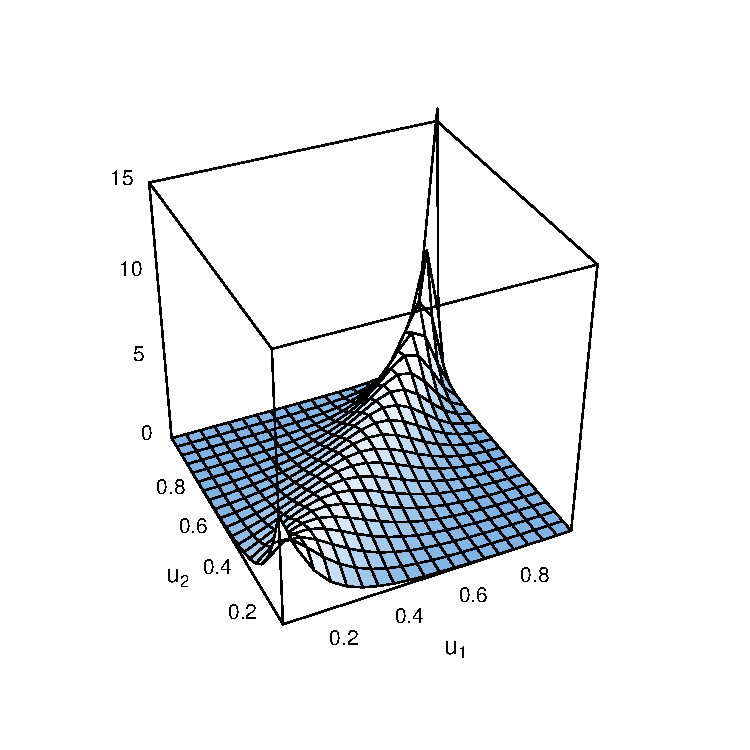
\includegraphics[trim= 1.8cm 1cm 2cm 1cm, clip=true, width = .32\textwidth]{Figures/Fig-1-2/gumbel-dens.pdf}
	}
	\hfill
	\subfloat{%
		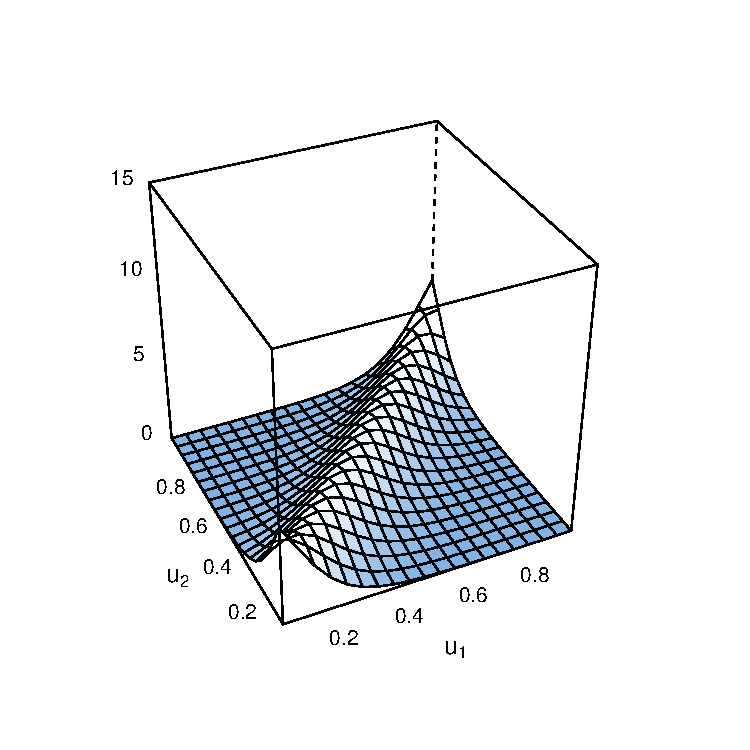
\includegraphics[trim= 1.8cm 1cm 2cm 1cm, clip=true, width = .32\textwidth]{Figures/Fig-1-2/frank-dens.pdf}
	}
	\hfill
	\subfloat{%
		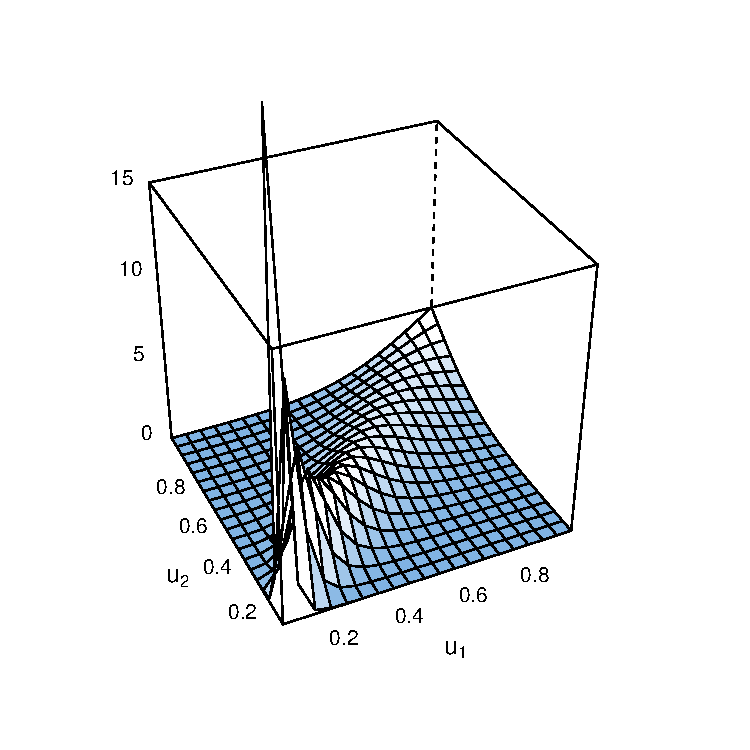
\includegraphics[trim= 1.8cm 1cm 2cm 1cm, clip=true, width = .32\textwidth]{Figures/Fig-1-2/clayton-dens.pdf}
	}
	\hfill
	\subfloat{%
		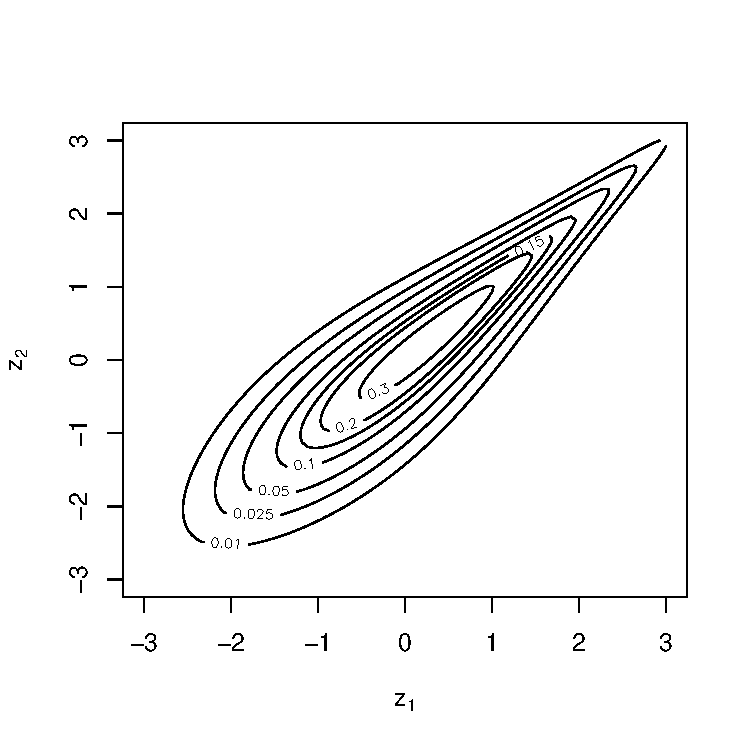
\includegraphics[trim= 0cm 0cm 0cm 2cm, clip=true, width = .32\textwidth]{Figures/Fig-1-2/gumbel-contour.pdf}
	}
	\hfill
	\subfloat{%
		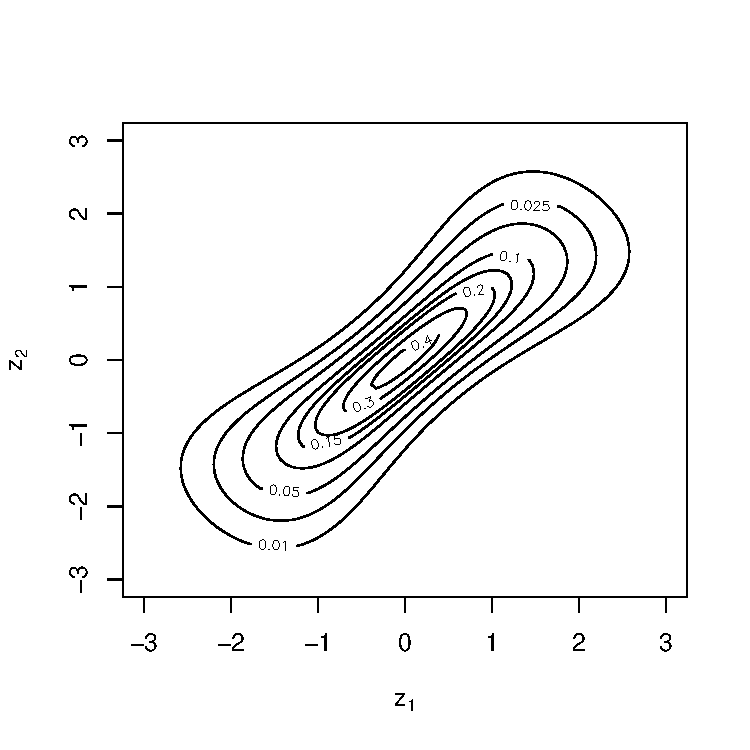
\includegraphics[trim= 0cm 0cm 0cm 2cm, clip=true, width = .32\textwidth]{Figures/Fig-1-2/frank-contour.pdf}
	}
	\hfill
	\subfloat{%
		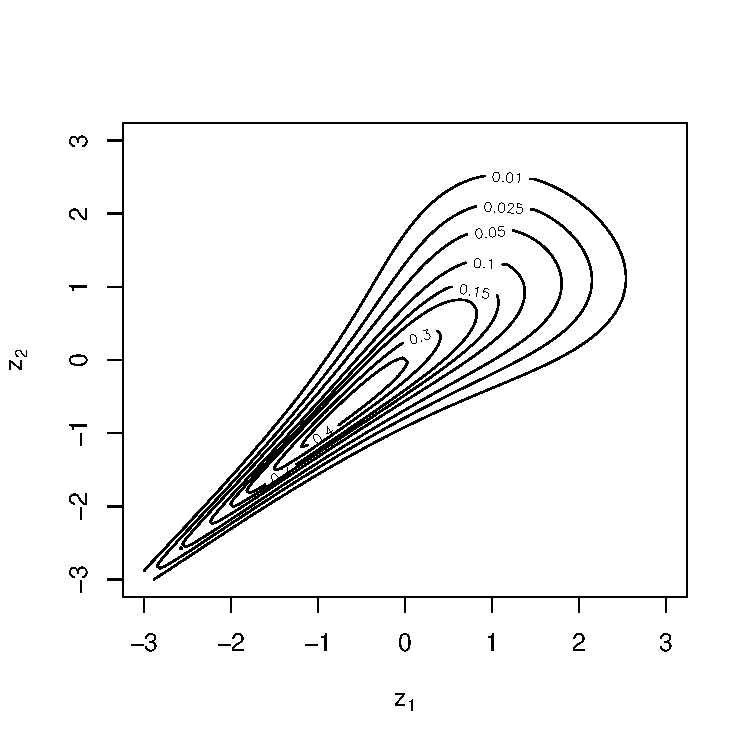
\includegraphics[trim= 0cm 0cm 0cm 2cm, clip=true, width = .32\textwidth]{Figures/Fig-1-2/clayton-contour.pdf}
}
	\caption[\textsc{Bivariate Archimedean copula densities:} A comparison between Gumbel, Frank and Clayton copulae]{\textsc{Bivariate Archimedean copula densities:} Top: three-dimensional density plots for theoretical Gumbel (left), Frank (middle) and Clayton (right) copulae. The parameters have been chosen in such a way that Kendall's $\tau = 0.7$. Below are the respective contour plots belonging to the densities.}
	\label{dens-cont-arch}
\end{figure}


\section{Dependence measures}

We will now, first, introduce the concept of the aforementioned tail dependence and, second, describe two ways to quantify the existence, direction and strength of dependence between two random variables and their connection to the dependence structure of a copula. The first of which will be \textit{Kendall's Tau} and the second \textit{Blomqvist's Beta}. There also exists a variety of other dependence measures; for the sake of simplicity, however, we will only present those needed for our simulation study. 

\subsubsection*{Tail dependence}

The concept of tail dependence arises from extreme value theory and quantifies the joint presence of either very small or very large values or both via a tail-dependence-coefficient. Given two random variables $X_1$ and $X_2$ it is defined by the limit

\begin{equation}
	\lambda^{\mathrm{u}}=\lim _{q \rightarrow 1^{-}} P\left(X_{2}>F_{2}^{-1}(q) \mid X_{1}>F_{1}^{-1}(q)\right)=\lim _{q \rightarrow 1^{-}} \frac{1-2 q+C(q, q)}{1-q} 
\end{equation}
%
for upper tail dependence and

\begin{equation}
	\lambda^{\mathrm{l}}=\lim _{q \rightarrow 0^{+}} P\left(X_{2} \leq F_{2}^{-1}(q) \mid X_{1} \leq F_{1}^{-1}(q)\right)=\lim _{q \rightarrow 0^{+}} \frac{C(q, q)}{q}
\end{equation}
%
for lower tail dependence. The coefficient's support is on $0 \leq \lambda^{\mathrm{u}},\lambda^{\mathrm{l}} \leq 1 $ and can be understood as a measure of strength, getting closer to one, the closer the link between X reaching large values and Y reaching large values likewise. A more detailed introduction into extreme value theory can be found in Chapter 7 of \citet{mcneil2015quantitative}.

\subsubsection*{Kendall's Tau}

\textit{Kendall's Tau} \citep*{kendall1938new} is a rank based correlation coefficient that splits the present data into concordant or discordant pairs and calculates its difference. Suppose there is a set of $x$-sorted observations $\left(x_i , y_i \right)$ for $ i \in \left\lbrace 1,\dots ,n \right\rbrace $ and $x_1 <x_2 < \dots < x_n$, then two pairs of variables $\left( x_i , y_i \right) $ and $\left( x_j , y_j \right)$ for $i<j$ are called \textit{concordant} if either both $x_i > x_j$ and $y_i > y_j$ or $x_i < x_j$ and $y_i < y_j$, otherwise they are called \textit{discordant}.

The product of their differences is summed up and divided by $ {n\choose 2} = \frac{n(n-1)}{2}$ to build the empirical $\tau$-coefficient defined as

\begin{equation}
	\label{emp-kendall}
		\hat{\tau}:=\frac{2}{n(n-1)} \sum_{i<j} \mathrm{sgn}\left(x_{i}-x_{j}\right) \mathrm{sgn}\left(y_{i}-y_{j}\right)
\end{equation}
%
with $ \mathrm{sgn}\left(\cdot \right) $ being the signum function. $\hat{\tau}$ can take any value in $\left[ -1,1 \right] $ where $-1$ and $+1$ imply perfect negative or positive dependence respectively. The provided formula above does not allow for ties where $\mathrm{sgn}\left(x_{i}-x_{j}\right) \mathrm{sgn}\left(y_{i}-y_{j}\right) = 0$. Kendall's Tau is directly connected to the bivariate copula distribution via (see Appendix \ref{AppendixA} for proof)

\begin{equation}
	\label{tau-copula}
		\tau=-1+4 \int_{[0,1]^{2}} C\left(u_{1}, u_{2}\right) \mathrm{d} C\left(u_{1}, u_{2}\right) .
\end{equation}

The fact that Kendall's Tau is solely dependent on the copula allows us to estimate the copula parameter $\theta$ via the inverse of \ref{tau-copula} such that $\tau (C_\theta) = \hat{\tau}$. This will be discussed in more detail when we introduce the copula estimators for our simulation in Chapter 2.

\subsubsection*{Blomqvist's Beta}

An even simpler way to measure bivariate dependence is the use of \textit{Blomqvist's Beta}, first described by \citet{blomqvist1950measure}. The idea is to divide the data plane into four quadrants and count all respective observations via a $2 \times 2$ contingency matrix. From this Blomqvist's $\beta$ is constructed as follows:

Let $\tilde{X}$ and $\tilde{Y}$ be the respective medians of two random variables $X_1, \dots , X_n$ and $Y_1, \dots , Y_n$. To construct a useful measure of dependence, the $x-y$ plane is then divided into four parts by splitting it at $x=\bar{X}$ and $y=\bar{Y}$ and counting all points that lie in diagonally opposing quadrants. We then define $n_1$ as the number of points in the lower left and upper right region and $n_2$  as the number of points in the upper left and lower right region to construct the empirical Blomqvist's Beta

\begin{equation}
	\hat{\beta}=\frac{n_{1}-n_{2}}{n_{1}+n_{2}}=\frac{2 n_{1}}{n_{1}+n_{2}}-1 ,
\end{equation}
%
where $-1\leq \hat{\beta} \leq 1$. For an odd sample size, either one or two points must lie on one or both segmenting lines $x=\tilde{X}$ and $y=\tilde{Y}$ respectively, which raises the question to which quadrant the point will be counted. Blomqvist suggests that for one point lying on a median line, it shall be ignored, while in the case of two points lying on both segmenting lines, one is ignored and the second is counted to the quadrant both points adjoin.

From the population analogue of Blomqvist's Beta 

\begin{equation}
	\beta=P\{(X-\tilde{X})(Y-\tilde{Y})>0\}-P\{(X-\tilde{X})(Y-\tilde{Y})<0\} ,
\end{equation}
%
one can derive the Copula representation (done in Appendix \ref{AppendixA}) which is given by

\begin{equation}
	\label{beta-copula}
	\beta=4 C\left( F_{X}(\tilde{X}), F_{Y}(\tilde{Y})\right) -1 =4 C\left(\frac{1}{2}, \frac{1}{2}\right) -1
\end{equation}
%
This representation allows us estimate the copula parameter $\theta$ by solving the equation $\beta (C_\theta)=\hat{\beta}$. For both inversion methods it is assumed that $C \in C_\theta$ and $\theta \in \mathbb{R}$.